\documentclass[8pt]{extarticle}
\usepackage{helvet}
\usepackage[T1]{fontenc}
\usepackage[a4paper,landscape,margin=0.8cm]{geometry}
\usepackage[utf8]{inputenc}
\usepackage[english]{babel}
\usepackage{xcolor}
\usepackage{enumitem}

\usepackage{listings}
\usepackage{tcolorbox}
\tcbuselibrary{breakable}
\tcbuselibrary{skins}
\usepackage{caption}
\usepackage{multicol}
\usepackage{graphicx}
\graphicspath{{./images/}}

\BeforeBeginEnvironment{lstlisting}{\begin{tcolorbox}[boxsep=-3mm]}
\AfterEndEnvironment{lstlisting}{\end{tcolorbox}}

\lstset{basicstyle=\tiny}

\renewcommand{\familydefault}{\sfdefault}

\let\oldtextbf\textbf
\renewcommand{\textbf}{\tiny\oldtextbf}

\parindent0pt

\begin{document}
\begin{multicols*}{5}
	\textbf{[Betriebssystem API]}\\
	\textbf{ProzessorPrivilege Level}
	Kernel Mode, User Mode. OS läuft üblicherweise im Kernel Mode aber auch hier werden bestimmte Prozesse im User Mode ausgeführt.\\\\
	\textbf{Micro Kernel}
	Kernelfunktionalität auf Minimum reduziert. Nur Kritische teile des Kernels laufen im Kernel-Mode. Vorteil: Stabilität, Analysierbarkeit. Nachteil: Performance-Einussen durch häufigen Mode-Wechsel.\\\\
	\textbf{Monolithische Kernel}
	Meiste OS-Kernel sind monolithisch. Viel Funktionalität auch im Usermode -> weniger Mode Wechsel dafür weniger Schutz vor Programmierfehlern.
	\textbf{Unikernel}
	Kernfunktionalität als Library. Keine Trennung Kernel-/User-Mode. Sehr Minimal und Kompakt. Nur ein Programm läuft.\\
	\textbf{Programmargumente}
		
	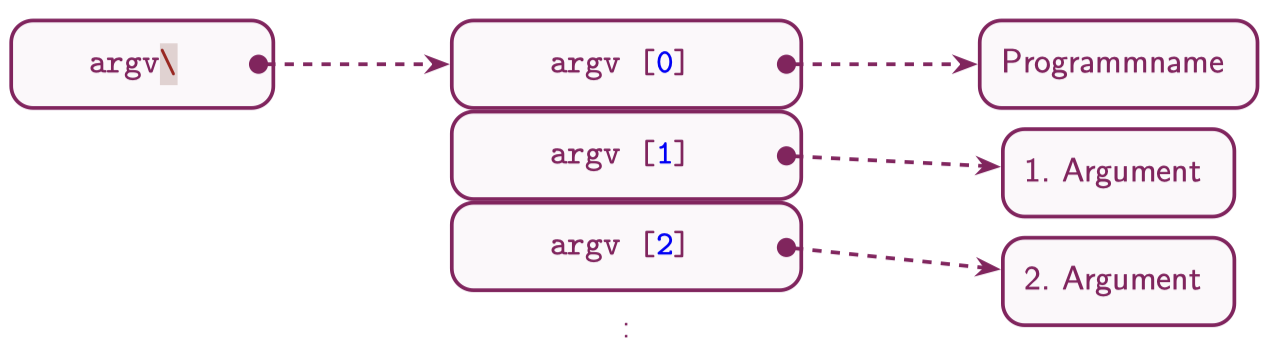
\includegraphics[scale=0.24]{Programmargumente.png}
	\textbf{ABI-Kompatibilität} Linux-Kernel sind nicht binär-kompatibel Z.B. Kernel A: exit hat Code 60 und erwartet Exit-Code in Register al Z.B. Kernel B: exit hat Code 55 und erwartet Exit-Code in Register al
	\textbf{Umgebungsvariablen} werden implizit bereitgestellt. Eignet sich für Informationen werlche immer gleich sind.
	\begin{lstlisting}
PATH=/usr/home
	\end{lstlisting}
	Key=Value. Jeder Key höchstens einmal. Umgebungsvariablen werden vom erzeugenden Prozess festgelegt z.B. von der Shell. Umgebunsvars sind array "environ" abgelegt. Zugriff mit \texttt{getenv, putenv, setenv, unsetenv}.
	\textbf{Abfragen} \texttt{char *value = getenv("PATH");}
	\textbf{Setzen} \texttt{int ret = setenv("HOME", "/usr/home", 1);}
	\textbf{Entfernen} \texttt{int ret = unsetenv("HOME");}
	\textbf{Hinzufügen} \texttt{int ret = putenv("HOME=/usr/home");}\\\\
	\rule{\linewidth}{0.4pt}
	\textbf{[Filesystem API]}\\
	Datei besteht aus Daten und Metadaten.
	\textbf{Dateitypen} haben für FS und OS fast keine Relevanz. Es liegt an der Applikation den Datentyp richtig zu bestimmen, diese müssen die Daten validieren.\\\\
	\textbf{Verzeichnis Begriffe}
	\begin{itemize}[noitemsep, topsep=0pt, leftmargin=*]
		\item Verzeichnis: Liste die Dateien oder Verzeichnisse enhält. Als Datei realisiert
		\item Verzeichnishiereachie: Gesamtheit aller Verzeichnisse im System. Jedes Verz. hat genau ein parent (ausser root).
		\item Wurzelverzeichnis: Oberstes Verzeichnis. Keinen Namen "/".
	\end{itemize}
	Zwei Referenzen pro Verzeichis: "." auf sich selbst, ".." auf parent. Jeder Prozess hat ein Arbeitsverzeichnis. \texttt{getcwd (get current working directory), chdir (change directory)}\\\\
	\textbf{Pfade}
	\begin{itemize}[noitemsep, topsep=0pt, leftmargin=*]
		\item Absoluter Pfad beginnt mit /
		\item Realtiver Pfad beginnt nicht mit /
		\item Kanonischer Pfad sind absolut ohne "." und ".."
	\end{itemize}
	Limitierungen sind in \texttt{<limits.h>} festgelegt\\
	\textbf{Zugriffsrechte} \texttt{0740 oder rwxr-----} Owner hat alle Rechte, Gruppe nur Lesen, Andere keine
	\textbf{POSIX-API} API für direkten, unformatierten Zugriff auf Inhalt der Datei.
	\textbf{File Descriptor}
		
	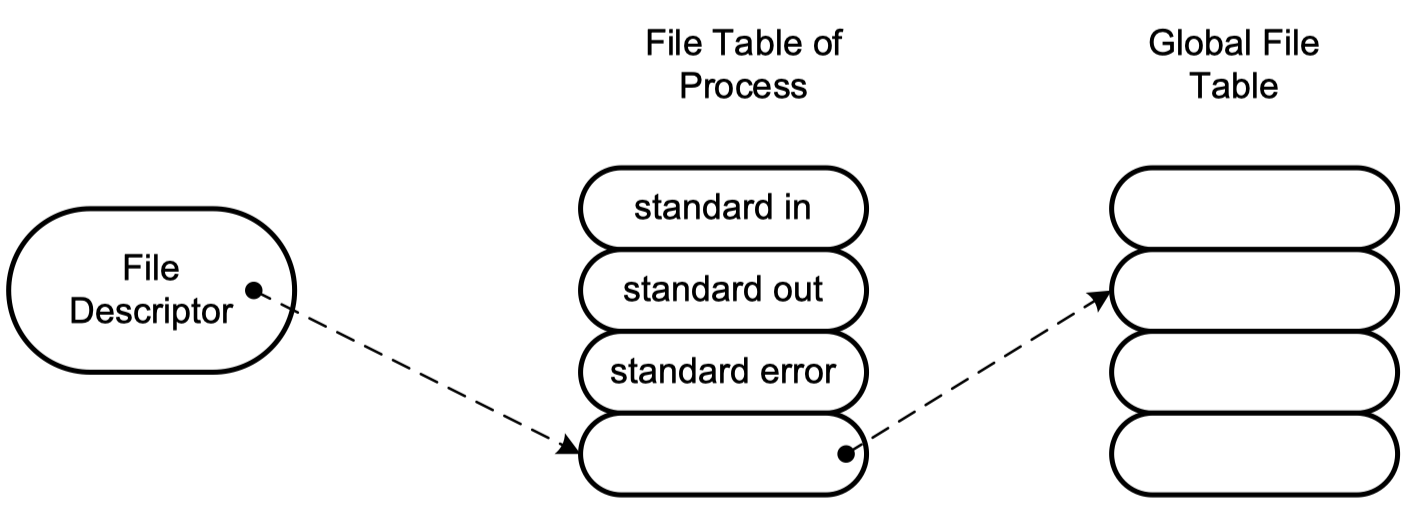
\includegraphics[scale=0.2]{File_Descriptor.png}\\
	Gilt immer nur innerhalt eines Prozesses. Tabelle mit allen geöffneten Dateien im Prozess zeigt auf globale Tabelle. Enthält Daten, um physische Datei (mit richtigem Treiber, Datenträger, etc) zu identifizieren.\\
	% TODO API Methoden einfügen?!
	\textbf{C-API} Unabhängig von Betriebssystem, Streambasiert, anderes Error-Handling\\\\
	\rule{\linewidth}{0.4pt}
	\textbf{[Prozesse]}\\
	Umfasst das Abbild eines Programms im Hauptspeicher, die globalen Variablen des Programms, Speicher für Heap und Stack. 
	\begin{itemize}[noitemsep, topsep=0pt, leftmargin=*]
		\item Programm: passiv, beschreibt bestimmte Abläufe
		\item Prozess: aktiv, führt Abläufe aus
	\end{itemize}
	\textbf{Process Control Block (PCB)} ist ein Speicher für alle Daten, die das OS benötigt, um die Ausführung des Prozesses ins Gesamtsystem zu integrieren, u.a.: ID, Parent ID, Zustands, Scheduling-Infos,...
		
	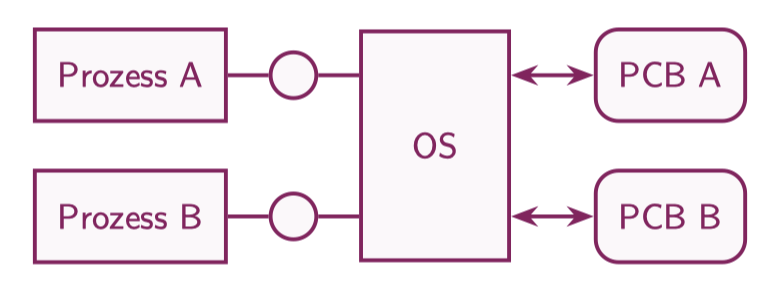
\includegraphics[scale=0.3]{PCB.png}\\
	\textbf{Interrupts} dabei muss der Kontext des aktuellen Prozesses im PCB gesichert werden (context save). Gesichert wird: Register, Flags, Instruction Pointer, MMU-Konfiguration. Danach wird der \textbf{Interrupt-Handler} aufgerufen, dieser kann den Kontext komplett überschreiben, danach wird der Kontext des Prozesses aus dem PCB wiederhergestellt (context restore).\\\\
	\textbf{Prozess erzeugen} Das OS muss 1. Einen Prozess erzeugen 2. Ein Programm in den Prozess laden
	\textbf{Prozess-Hierarchie} Jeder Prozess hat 1 Parent und beliebig viele childs: \texttt{pstree} zum anzeigen\\\\
	\textbf{Fork} Erzeugt exakte Kopie des Prozesses mit eigener Prozess-ID
	\begin{itemize} [noitemsep, topsep=0pt, leftmargin=*]
		\item Bei Erfolg: Gibt die Prozess-ID von C zurück (> 0)
		\item Bei Misserfolg: Gibt -1 zurück und Fehlercode in errno
	\end{itemize}
	\begin{lstlisting}[language=c]
pid_t new_pid = fork();
if (new_pid > 0) {
	// Parent Code 
}
else if (new_pid == 0) {
	// Child Code
}

void spawn_worker() {
    if (fork() == 0) {
        // Child process
        // Perform some tasks in the worker
        exit(0); // Exit from the worker
    }
}
	\end{lstlisting}
	\begin{itemize} [noitemsep, topsep=0pt, leftmargin=*]
		\item \texttt{pid\_t wait (int *status)}: Unterbricht den aufrufenden Prozess und wartet bis einer seiner Child-Prozesse beendet wurde.
		\item \texttt{pid\_t waitpid (pid\_t pid, int *status, int options)}: Gleich wie wait der pid bestimmt aber auf welchen prozess man warten will
		\item \texttt{void exit (int code)}: Kann an jeder Stelle im Programm verwendet werden und bietet somit eine Alternative zum «Rücksprung» aus main
	\end{itemize}
	\vspace{5pt}
	\textbf{exec-Funktionen} Jede exec-Funktion ersetzt im gerade laufenden Prozess das Programmimage durch ein anderes Programmimage.\\\\
	\textbf{Zusammenspiel}
			
	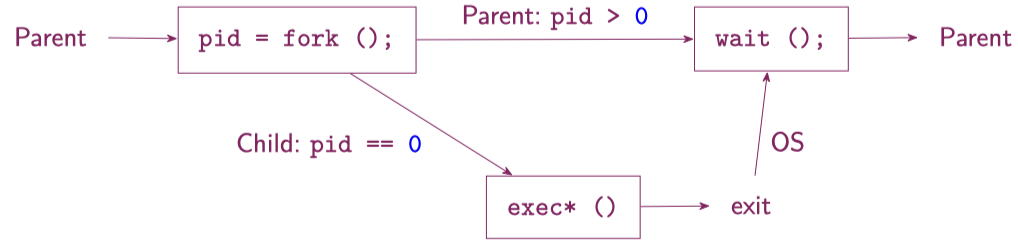
\includegraphics[scale=0.299]{Prozesse.png}
	\textbf{Zombie-Prozess} Der Parent-Prozess muss auf jeden Fall wait aufrufen um auf den Child-Prozess zu warten. Child ist zwischen seinem Ende und dem Aufruf von wait durch P ein Zombie-Prozess («tot, aber noch nicht entfernt»). Wird wait über längere Zeit nicht aufgerufen, dann muss P gestoppt werden.
	\textbf{Orphan-Prozess}
	Beim Ende eines Prozesses werden alle seine Child-Prozesse an den Prozess mit der pid = 1 übertragen. Dieser ruft in Endlosschleife \texttt{wait} auf.
	\textbf{Lesen von PIDs}:
	\begin{lstlisting}
#include <stdio.h>
#include <unistd.h>

int main()
{
    pid_t my_pid = getpid();
    pid_t my_parent_pid = getppid();
}
	\end{lstlisting}\
			
	\rule{\linewidth}{0.4pt}
	\textbf{[Programme und Bibliotheken]}\\
	\textbf{C-Toolchain}
		
	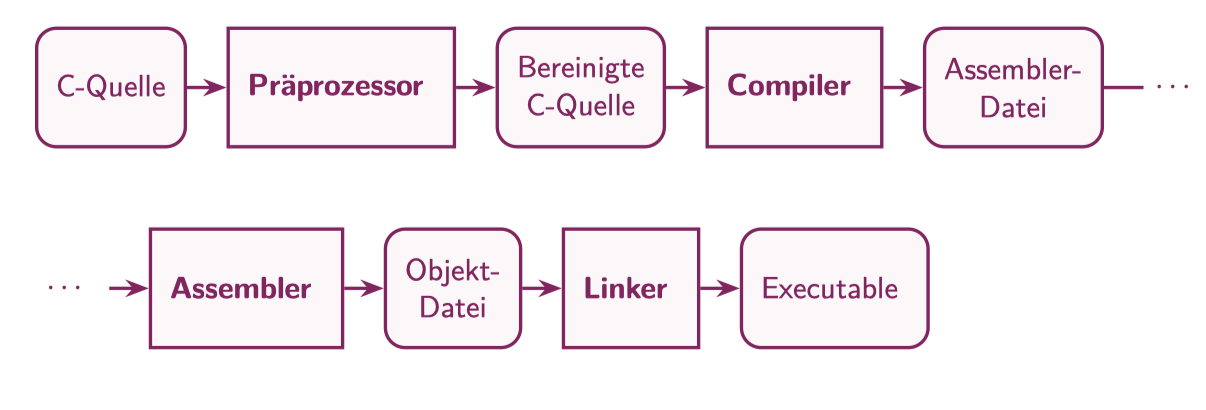
\includegraphics[scale=0.255]{C-Toolchain.png}
	Der \textbf{Präprozessor} gibt eine reine C-Datei aus, ersetzt Makros, entfernt Kommentare und Präprozessor-Direktiven. Der \textbf{Linker} verknüpft Objekt-Dateien zu Executables oder dynamischen Bibliotheken, Löst Referenzen der Objektdateien soweit wie möglich auf(Executables und dynamische Bibliotheken müssen vollständig aufgelöst sein).\\\\
	\textbf{Loader} lädt Executables und dynamische Bibliotheken in den Hauptspeicher\\\\
	\textbf{ELF, Executable and Linking Format} ist ein Binär-Format das Kompilate spezifiziert. Hat zwei Views:
	\begin{itemize} [noitemsep, topsep=0pt, leftmargin=*]
		\item Linking View
		\item Execution View
	\end{itemize}
	\vspace{5pt}
	\textbf{ELF Struktur} besteht aus verschiedenen Bereichen: Header, Program Header Table(Execution View), Segmente(Execution View), Section Header Table(Linking View), Sektionen(Linking View).
			
	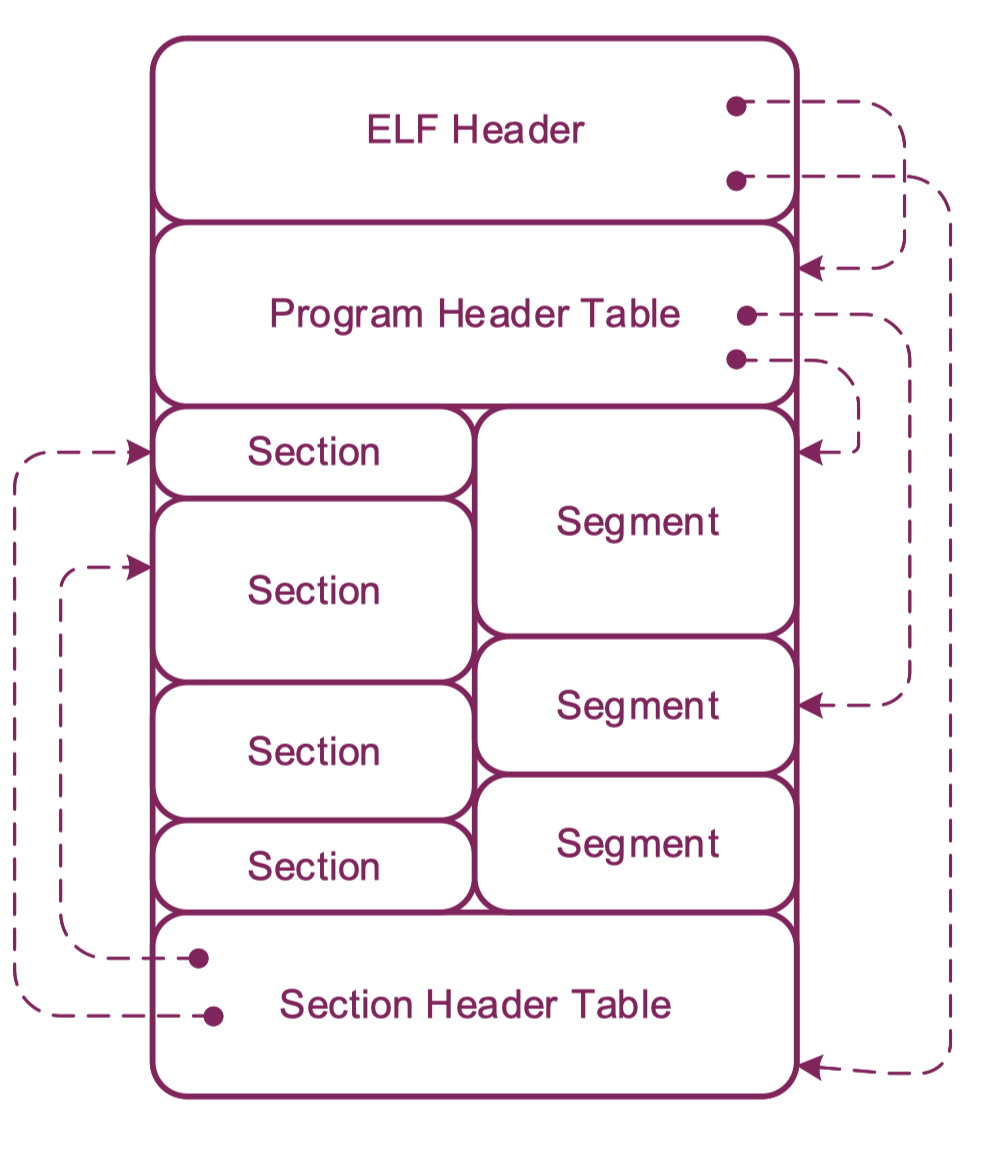
\includegraphics[scale=0.2]{ELF.png}
	%TODO wenn platz am Schluss bild einfügen "ELF screenshot"
			
	Der \textbf{Header} beschreibt den Aufbau der Datei: Typ, 32-/64-bit, Encoding (Little-/Big-endian),Maschine, Entrypoint Adresse, Relative Adresse der Program und Section Header Table.\\
	• \textbf{Program Header Table} mit n Einträgen je 32 Byte welche jeweils ein Segment Beschreiben. Die Segmente werden vom Loader zur Laufzeit verwendet\\
	• \textbf{Section Header Table} mit m Einträgen pro 40 Byte beschreiben eine Sektion. Sektionen werden vom Linker verwendet.\\
	%TODO beispielsektionen noch einfügen
	• \textbf{String Tabelle} Bereich in Datei der null-terminierte Strings enthält (typischerweise Namen von Symbolen). Strings werden relativ zum Beginn der Tabelle referenziert.\\
			
	\textbf{Statische Bibliotheken} sind Archive von Objekt-Dateien
	\begin{itemize} [noitemsep, topsep=0pt, leftmargin=*]
		\item Linker behandelt statische Bibliotheken wie mehrere Objekt-Dateien
		\item Alle gelinkten statischen Bibliotheken werden vom Linker im Programm-Image verteilt
		\item Alle Variablen und Funktionen werden auf absolute Adressen fixiert
	\end{itemize}
	Statische Bibliotheken sind einfach zu implementieren
	\begin{itemize} [noitemsep, topsep=0pt, leftmargin=*]
		\item Nachteil: Bei Änderung in Bibliothek muss Programm neu erstellt werden, Pulgins sind nicht möglich.
	\end{itemize}
	\textbf{Dynamische Bibliotheken}  
	\begin{itemize} [noitemsep, topsep=0pt, leftmargin=*]
		\item Dynamische Bibliotheken: Linken erst zur Ladezeit bzw. Laufzeit des Programms
		\item Höherer Aufwand für Programmierer, Compiler, Linker und OS
		\item Executable enthält nur noch Referenz auf Bibliothek
	\end{itemize}
	Das Programm kann Updates erhalten ohne Binary zu ändern. Da Programm muss nur die Bibliothek laden die es braucht. Programme können um Funktionalität ergänzt werden.\\
	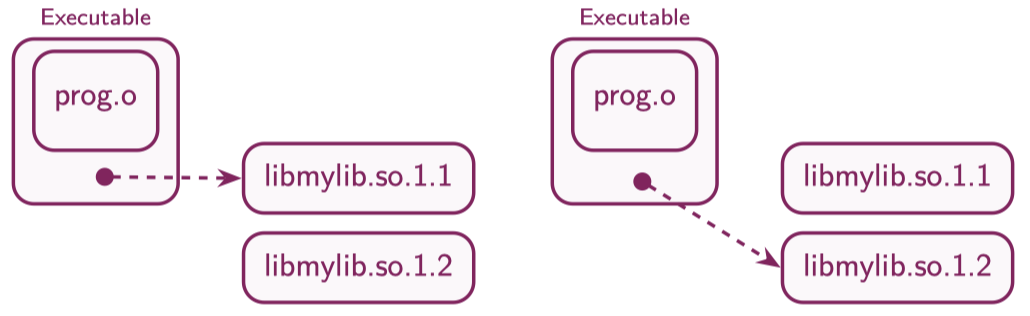
\includegraphics[scale=0.3]{Dynamische_Bibliotheken.png}
	\textbf{Implemetierung} Da gleiche Bibliotheken bei mehreren Programmen verwendet werden und der Code aber nicht mehrfach im Speicher abgelegt werden soll, hat jedes Programm eine eigene virtuelle Page für den Code.\\
			
	\begin{tabular}{|p{2.2cm}|p{2.2cm}|}
		\hline
		Position dependant Code                                                                                                                                                                                                              & Position Independant Code                                                                                                                                             \\
		\hline
		Code hängt normalerweise von absoluten Adressen ab (z.B. Funktionsaufrufe, Globale Variablen). Wird dieser code im Speicher verschoben stimmen die Referenzen nicht mehr. 
\includegraphics[scale=0.15]{Call_Position_dependant.png} & Verwendet nur Adressen relativ zum Instruction Pointer. 
\includegraphics[scale=0.15]{Call_Position_independant.png} x86\_64 hat relative Call- und Move-Instruktionen \\
		\hline
	\end{tabular}
	\textbf{POSIX Shared Objects API}
	\begin{itemize} [noitemsep, topsep=0pt, leftmargin=*]
		\item \texttt{void * dlopen (char * filename, int mode)} Öffnet dynamische Bibliotheken und gibt Handle darauf zurück
		\item \texttt{void * dlsym (void * handle, char * name)} Gibt die Adresse des Symbols name aus der mit handle bezeichneten Bibliothek zurück
		\item \texttt{int dlclose (void * handle)}
		\item \texttt{char * dlerror ()}
	\end{itemize}
	Shared Objects können automatisch bei Bedarf geladen werden, hierfür braucht es eine Referenz im ELF auf das SO.
			
	\textbf{Benennungsschema}
			
	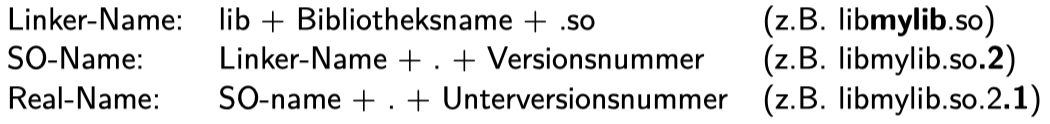
\includegraphics[scale=0.29]{Benennungschema_Shared_Objects.png}\\\\
	\rule{\linewidth}{0.4pt}
	\textbf{[Threads]}\\\\
	\textbf{Prozessmodell} Jeder Prozess hat virtuell den ganzen Rechner für sich alleine (Adressraum, Register, Isolation). Gut für unabhängige Applikationen.
			
	•	Nachteile: Overhead für Prozesserzeugung, Erschwerte gemeinsame Ressourcennutzung, Parallele Abläufe innerhalb derselben Applikation aufwändig.\\\\
	\textbf{Threadmodell} Threads sind parallel ablaufende Aktivitäten innerhalb eines Prozesses. Haben auf alle Ressourcen gleichermassen Zugriff: Code (text section) Globale Variablen (data section) Heap Geöffnete Dateien MMU-Daten.
	\textbf{Stack} Jeder Thread benötigt einen eigenen Kontext und Stack.\\\\
	\textbf{Amdahls Law}\\
	N = number of processors used
				
	p = proportion of the computation that can be parallelized zwischen 0 und 1
				
	s = serieller Anteil
				
	Speedup = 1/[(1-P ) + (P/N)]
	
	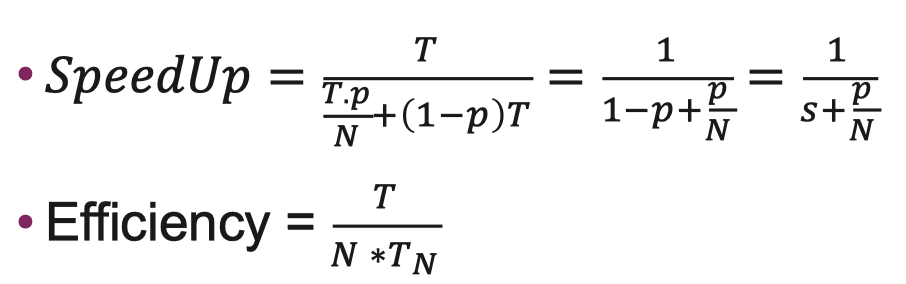
\includegraphics[scale=0.3]{amdahl.png}\\\\
	\textbf{POSIX Thread API}
	\begin{lstlisting} [language=c]
int pthread_create (
	pthread_t *thread_id,
	pthread_attr_t const *attributes,
	void * (*start_function) (void *),
	void *argument)
	\end{lstlisting}
	\begin{itemize} [noitemsep, topsep=0pt, leftmargin=*]
		\item Die erste Instruktion, die der neue Thread ausführen soll, ist ein Aufruf der Funktion, deren Adresse in \texttt{start\_function} übergeben wird.
		\item Zusätzlich übergibt der Thread das Argument \texttt{argument} an diese Funktion.
		\item Es liegt völlig in der Verantwortung des Programmierers, dass \texttt{argument} und \texttt{start\_function} zusammenpassen; das OS reicht die Adresse lediglich weiter.
		\item \texttt{argument} ist typischerweise ein Pointer auf eine Datenstruktur auf dem Heap.
	\end{itemize}
	Die \textbf{Lebensdauer eines Threads} ist solange bis dieser aus \texttt{start\_function} zurückspringt, \texttt{pthread\_exit} aufruft, ein anderer Thread \texttt{pthread\_cancel} aufruft oder der Prozess beendet wird.\\\\
	\textbf{Methoden}
	\begin{itemize} [noitemsep, topsep=0pt, leftmargin=*]
		\item \texttt{void pthread\_exit (void *return\_value)} Beendet den Thread und gibt den return\_value zurück.
		\item \texttt{int pthread\_cancel (pthread\_t thread\_id)} Sendet eine Anforderung, dass der Thread mit thread\_id beendet werden soll.
		\item \texttt{int pthread\_detach (pthread\_t thread\_id)} Entfernt den Speicher, den ein Thread belegt hat, falls dieser bereits beendet wurde.
		\item \texttt{int pthread\_join (pthread\_t thread\_id, void **return\_value)} Wartet solange, bis der Thread mit thread\_id beendet wurde.
		\item \texttt{pthread\_t pthread\_self (void)} Gibt die ID des gerade laufenden Threads zurück.
	\end{itemize}
	\vspace{5pt}
	\textbf{Thread-Local Storage}
	\begin{itemize} [noitemsep, topsep=0pt, leftmargin=*]
		\item TLS ist ein Mechanismus, der globale Variablen per Thread zur Verfügung stellt
		\item Auf OS-Ebene braucht man dafür mehrere explizite Einzelschritte:
		\item Bevor Threads erzeugt werden:
		\item \begin{enumerate}[noitemsep, topsep=0pt, leftmargin=*]
		\item Anlegen eines Keys, der die TLS-Variable identifiziert
		\item Speichern des Keys in einer globalen Variable
		\end{enumerate}
		\item Im Thread:
		\item \begin{enumerate}[noitemsep, topsep=0pt, leftmargin=*]
		\item Auslesen des Keys aus der globalen Variable
		\item Auslesen / Schreiben des Werts anhand des Keys über besondere Funktionen
		\end{enumerate}	
	\end{itemize}
	
	\vspace{5pt}
	
	\rule{\linewidth}{0.4pt}
	\textbf{[Scheduling]}\\
	
	\textbf{Zustände eines Threads}: running(pro Prozessor immer nur einer), ready, waiting (wartet auf Ereignis)
	
	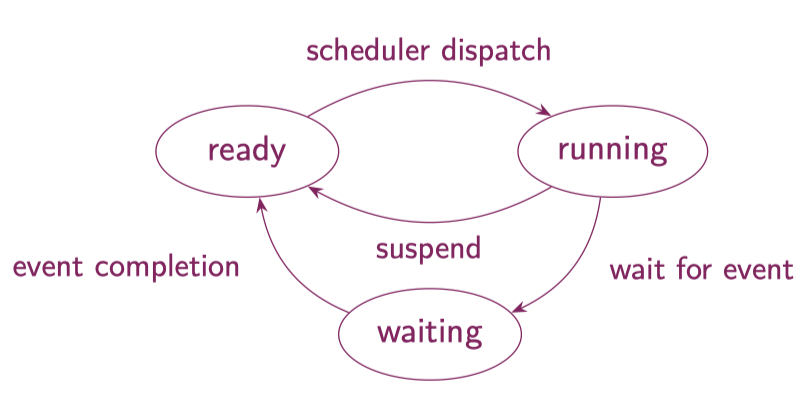
\includegraphics[scale=0.32]{Thread_Grundmodell.png}
	\textbf{Wartende Threads} müssen die nicht im Busy-Wait machen, OS registriert auf das zu wartende Ereignis und setzt den thread in den Zustand \texttt{waiting}. Wenn das Ereignis eintritt setzt das OS den Zustand auf \texttt{ready}.\\

	In der \textbf{Ready-Queue} befinden sich alle laufbereiten Threads. Neue Threads kommen typischerweise direkt in die Ready-Queue.\\
	
	Wenn kein Thread laufbereit ist, schaltet das OS den Prozessor in den \textbf{Powerdown-Modus}. Busy-Waits verhindern diesen Mechanismus.\\
	
	\textbf{Arten von Threads}
	\begin{itemize} [noitemsep, topsep=0pt, leftmargin=*]
		\item I/O-lastig
		\item Prozessor-lastig
	\end{itemize}
	
	\vspace{5pt}
	
	\textbf{Arten der Nebenläufigkeit}
	\begin{itemize} [noitemsep, topsep=0pt, leftmargin=*]
		\item Kooperativ, jeder Thread entscheidet selbst wann er den Prozessor abgibt
		\item \textbf{Präemptiv}, Der Scheduler entscheidet\\Der aktuelle Thread läuft so lange weiter bis: Auf I/O wartet, auf Thread/Ressource wartet, Timer-Interrupt, Neuer Thread bevorzugt werden soll
	\end{itemize}
	
	\vspace{5pt}
	
	\textbf{Bursts}
	
	Prozessor-Burst -> Intervall, in dem ein Thread den Prozessor in einem parallelen System voll belegt, also vom Eintritt in running bis zum nächsten waiting.
	
	I/O-Burst -> Intervall, in dem ein Thread den Prozessor nicht benötig, also vom Eintritt in waiting bis zum nächsten running\\
	
	\textbf{Anforderungen an Scheduler}\\
	\underline{aus Andwendungssicht:}
	Durchlaufzeit (turnaround time): Zeit vom Starten des Threads bis zu seinem Ende\\
	Antwortzeit (response time): Zeit vom Empfang eines Requests bis die Antwort zur Verfügung steht\\
	Wartezeit (waiting time): Zeit, die ein Thread in der Ready-Queue verbringt\\
	\underline{aus Systemperspektive:}
	Durchsatz (throughput): Anzahl Threads, die pro Intervall bearbeitet werden\\
	Prozessor-Verwendung (processor utilization): Prozentsatz der Verwendung des Prozessors gegenüber der Nichtverwendung\\
	
	\textbf{FCFS-Strategie}\\
	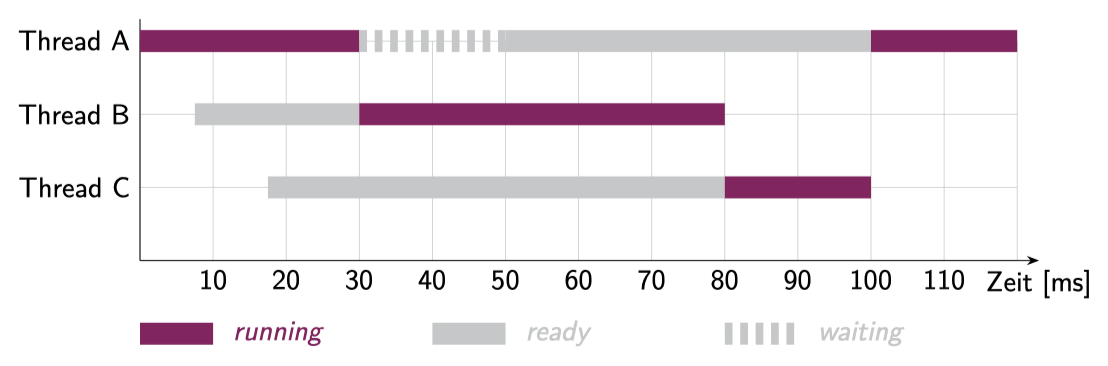
\includegraphics[scale=0.29]{FCFS_Scheduling.png}
	Threads werden in der Reihenfolge hinzugefügt, in der sie der Ready-Queue hinzugefügt wurden (FIFO). Ist nicht präemtiv, Threads geben Prozessor nur ab wenn sie \texttt{waiting} sind oder sich beenden.\\
	
	\textbf{SJF-Strategie (Shortest Job First}\\
	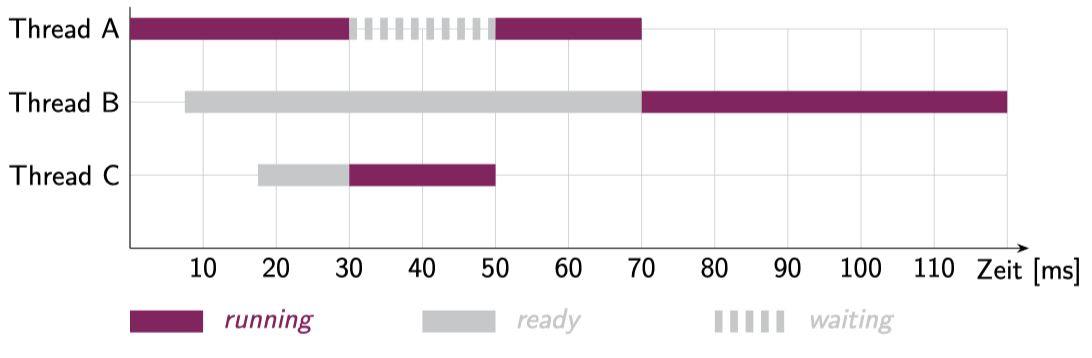
\includegraphics[scale=0.29]{SJF_Scheduling.png}
	Wählt den Prozess aus der den nächsten kürzesten Prozessor-Burst hat. Bei gleicher Länge: FCFS. Kooperativ und Präemptiv möglich.
	Diese Strategie ergibt die optimale Wartezeit.\\
	\underline{Die Schwierigkeit} besteht darin zu wissen wie lange der Burst sein wird, die Strategie kann nur mit Abschätzung historischer Daten annähernd implementiert werden.\\
	
	\textbf{Round-Robin-Scheduling}\\
	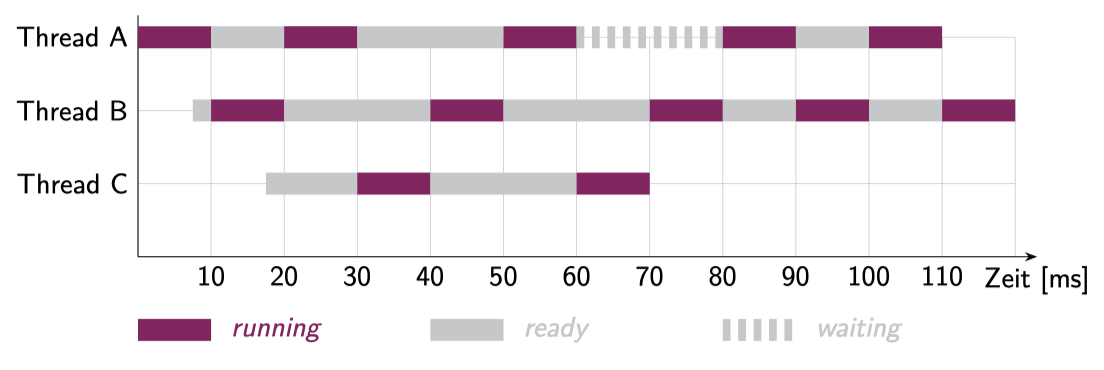
\includegraphics[scale=0.29]{RR_Scheduling.png}\\Time-Slice von 10ms\\
	Wie FCFS, jedoch kann ein Thread nur so lange wie sein Time-Slice laufen dann kommt er in die Ready-Queue. Bei füherer beendung kommt der nächste Thread früher.\\
	
	Bei \textbf{Prioritäten-barsiertem Scheduling} erhält jeder Thread eine Nummer mit deiner Priorität. Dabei werden Threads mit hoher Prio bevorzugt. \textbf{Starvation} kann bei diesem Prinzip auftreten\\
	
	Beim \textbf{Multi-Level Scheduling} werden Threads nach bestimmten Kriterien in Level aufgeteilt. Für jedes Level gibt es eine eigene Ready-Queue. Queues können unterschiedlich priorisiert werden oder auch Time-Slices erhalten. Beispiel:
	\begin{itemize} [noitemsep, topsep=0pt, leftmargin=*]
		\item 80\% für Vordergrund-Threads mit Round-Robin-Scheduling
		\item 20\% für Hintergrund-Threads mit First-Come-First-Served-Scheduling
	\end{itemize}
	
	\vspace{5pt}
	
	Bei \textbf{POSIX} haben Prozesse einen Nice-Wert (Auf Linux von -20 bis +19). Fehlerabfrage bei nice:
	\begin{lstlisting}[language=c]
errno = 0;
if (nice(i) == -1 && errno != 0) {
	// Error
} else {
	// -1 is nice value
}
		
	\end{lstlisting}
	
	\vspace{5pt}
	\rule{\linewidth}{0.4pt}
	\textbf{[Mutexe und Semaphoren]}\\\\
	\textbf{Inkrementierung in C}
	\begin{lstlisting}
mov rax, [counter]
inc rax
mov [counter], rax
	\end{lstlisting}
	Der Prozessor könnte zwischen den Instruktionen unterbrechen und den Thread wechseln. Dies kann unter Umständen zu einer \textbf{Race Condition} führen. Beim Kontextwechsel werden die Register gesichert, aber der Counter nicht. Wenn nebenläufige Threads auf den selben Hauptspeicher zugreifen passieren halt sachen.\\ Die \textbf{Critical Section} ist ein Codebreich in dem Daten mit anderen Threads geteilt werden.\\
	
	\textbf{Synchronisationsmechanismen} werden mit speziellen Instruktionen realisiert. Die Hardware garantiert, dass keine zwei dieser Instruktionen gleichzeitig ausgeführt werden, auch über mehrere Prozessoren hinweg:
	\begin{itemize} [noitemsep, topsep=0pt, leftmargin=*]
		\item \texttt{int test\_and\_set (int *target)} Liest den Wert von einer Adresse (0 oder 1) und setzt ihn dann auf 1
		\item \texttt{int compare\_and\_swap (int *a, int expected, int new\_a)} Liest einen Wert aus dem Hauptspeicher und überschreibt ihn im Hauptspeicher, falls er einem erwarteten Wert entspricht
	\end{itemize}
	\vspace{5pt}
	Ein \textbf{Semaphore} fungiert als Synchronisationsmechanismus und enthält einen Zähler. Die Funktion \texttt{post} erhöht den Zähler und \texttt{wait} verringert um 1 oder wartet falls der Zähler = 0 ist.
	\begin{lstlisting} [language=c]
#include <semaphore.h>
sem_t semaphore;

// Wait on the semaphore
sem_wait(&semaphore);

// Access the shared resource
sharedVariable++;
printf("Thread: %d\n", sharedVariable);

// Release the semaphore
sem_post(&semaphore);
	\end{lstlisting}
	\begin{itemize} [noitemsep, topsep=0pt, leftmargin=*]
		\item \texttt{sem\_trywait, sem\_timedwait} sind wie sem\_wait, brechen aber direkt ab falls Dekrement nicht möglich.
		\item \texttt{int sem\_destroy (sem\_t *sem);} Entfernt möglichen zusätzlichen Speicher von sem.
	\end{itemize}
	\vspace{5pt}
	
	Ein \textbf{Mutex} hat einen binären Zustand der nur mit \texttt{aqcuire} und \texttt{release} verändert werden kann.
	\begin{lstlisting}[language=c]
#include <stdio.h>
#include <pthread.h>

pthread_mutex_t mutex;

pthread_mutex_init (&mutex, 0);

pthread_mutex_lock(&mutex);
test_var ++;
pthread_mutex_unlock(&mutex);
	\end{lstlisting}
	\vspace{5pt}
	
	Bei \textbf{Priority Inversion} werden Gemeinsam verwendete Ressourcen im schlimmsten Fall mit der niedrigsten Priorität aller beteiligten Threads gehalten. Bei \textbf{Priority Inheritance} erhält der Thread der eine Ressource hält die höchste Priorität.\\
	
	\rule{\linewidth}{0.4pt}
	\textbf{[Signale, Pipes und Sockets]}\\
	
	\textbf{Signale} ermöglichen es, einen Prozess von aussen zu unterbrechen. Wird ein Signal geschickt verhält sich das OS wie bei einem Interrupt:
	\begin{enumerate}[noitemsep, topsep=0pt, leftmargin=*]
		\item Unterbrechen des gerade laufenden Prozesses (bzw. Threads)
		\item Auswahl der Signal-Handler-Funktion
		\item Ausführen der Signal-Handler-Funktion
		\item Fortsetzen des Prozesses (falls der Signal-Handler den Prozess nicht beendet)
	\end{enumerate}
	\underline{Quelle von Signalen} können Hardware/OS(Segmentation fault,...) oder andere Prozesse (kill command,...) sein.\\
	\begin{tabular}{|p{1cm}|p{3.5cm}|} %Achtung liste ist alles andere als vollständig
		\hline
		Signal & Beschreibung\\                                                                                                                                                                                                                                                                                                                                               
		\hline
		SIGFPE & Fehler in arithmetischer Operation\\
		\hline
		SIGILL & Ungültige Instruktion\\
		\hline
		SIGTERM & Die normale, höfliche Anfrage an den Prozess, sich zu beenden\\
		\hline
		SIGINT & Etwas nachdrücklichere Aufforderung Wird generiert, wenn der Benutzer Ctrl-C drückt\\
		\hline
		SIGTSTP & Versetzt einen Prozess in den Zustand stopped, ähnlich wie waiting Kann von der Shell mit Ctrl-Z ausgelöst werden\\
		\hline
	\end{tabular}\\
	\vspace{5pt}\\
	Von der \textbf{Shell} können Signale gesendet werden z.B.: \texttt{kill 1234 5678} sendet SIGTERM an Prozesse 1234 und 5678.\\
	
	\textbf{Signal-Handler ändern}:
	\begin{lstlisting}
struct sigaction {
	void (*sa_handler)(int);
	sigset_t sa_mask;
	int sa_flags;
};
	\end{lstlisting}
	\begin{itemize}[noitemsep, topsep=0pt, leftmargin=*]
		\item \texttt{sa\_handler} Adresse der Funktion welche beim Signal aufgerufen werden soll
		\item \texttt{sa\_mask} gibt an welche signale während handler-ausführung blockiert werden, das eigene immer.
		\item \texttt{sa\_flags} zusätzliche eigenschaften
	\end{itemize}
	\vspace{5pt}
	Eine \textbf{Pipe} ist eine Datei im Hauptspeicher die über zwei File-Deskriptoren verwendet wird. \texttt{read end} zum lesen aus der Pipe und \texttt{write end} zum Schreiben in die Pipe. Pipes ermöglichen Kommunikation über Prozessgrenzen hinweg.\\
	\textbf{Pipe erzeugen} %TODO rausnehmen falls am Schluss kein Platz
	\begin{lstlisting}[language=c] 
int fd[2];
pipe(fd);
int id = fork();

if (id == 0)
{                 // child
    close(fd[1]); // don't use write end
    char buffer[BSIZE];
    int n = read(fd[0], buffer, BSIZE);
}
else
{                 // parent
    close(fd[0]); // don't use read end
    char *text = "Hallo OST";
    write(fd[1], text, strlen(text) + 1);
}
	\end{lstlisting} 
	\begin{itemize}[noitemsep, topsep=0pt, leftmargin=*]
		\item Aus einer Pipe kann gelesen werden als ob sie eine Datei wäre
		\item Pipes sind unidirektional (nicht spezifiziert, was beim Schreiben ins read end oder Lesen vom write end passiert)
	\end{itemize}
	\vspace{5pt}
	\textbf{Sockets} sind eine Abstraktion über Kommunikationsmechanismen. Ein Socket repräsentiert einen Endpunkt auf einer Maschine.\\
	\texttt{int socket(int domain, int type, int protocol);} erzeugt neuen Socket als Datei. Gibt File-Deskriptor zurück.
	\begin{itemize}[noitemsep, topsep=0pt, leftmargin=*]
		\item \texttt{domain} ist die Adress-Domäne
		\begin{enumerate} [noitemsep, topsep=0pt, leftmargin=*]
			\item \texttt{AF\_UNIX}Innerhalb einer Maschine, Adressen = Pfade im Dateisystem
			\item \texttt{AF\_INET} Internet Kommunikation IPv4
			\item \texttt{AF\_INET6} Internet-Kommunikation IPv6/4
		\end{enumerate}
		\item \texttt{type} ist die Art der Kommunikation DGRAM = UPD, STREAM = TCP
		\item \texttt{protocol} systemspezifisch 0=default
	\end{itemize}
	\vspace{5pt}
	\textbf{Socket-Verwendung Client}
	\begin{enumerate} [noitemsep, topsep=0pt, leftmargin=*]
		\item Verbindung unter Angabe einer Adresse aufbauen: connect
		\item Senden von Daten (z.B. eine Anfrage): send oder write
		\item Empfangen von Daten (z.B. eine Antwort): recv oder read
		\item Schliessen der Verbindung: close
	\end{enumerate}
	
	\vspace{5pt}
	\textbf{Socket-Verwendung Server}
	\begin{enumerate} [noitemsep, topsep=0pt, leftmargin=*]
		\item Festlegen einer nach aussen sichtbaren Adresse: bind
		\item Bereitstellen einer Queue zum Sammeln von Verbindungsanfragen von Clients: listen
		\item Erzeugen eine Verbindung auf Anfrage von Client: accept (erzeugt neuen Socket)
		\item Empfangen von Daten (z.B. eine Anfrage): recv oder read
		\item Senden von Daten (z.B. eine Antwort): send oder write
		\item Schliessen der Verbindung: close
	\end{enumerate}
	%TODO Beispiele zur Angabe/Binden von Adressen weggelassen
	
	\vspace{5pt}
	\rule{\linewidth}{0.4pt}
	\textbf{[Message Passing und Shared Memory]}\\
	
	Beim \textbf{Message Passing} kann zwischen \textbf{fester} und \textbf{variabler} Nachrichtengrösse gewählt werden. Feste ist umständlicher zu verwenden, Variable ist aufwändiger zu implementieren.\\
	
	Bei \textbf{Direkter Kommunikation} werden Nachrichten von einem Prozess an einen anderen adressiert. Sender muss den Empfänger kennen \texttt{send (P2 , message)}. Bei Symmetrischer Kommunikation muss der Empfänger den Sender kennen \texttt{receive (P 1 , message)}, bei Asymmetrischer muss er ihn nicht Kennen, erhält ID in Out-Parameter \texttt{receive (id, message)}. Kommunikation nur zwischen zwei Prozessen.\\
	
	Bei \textbf{Indirekter Kommunikation} existieren spezifische OS-Objekte: Mailboxen, Ports oder Queues
	\begin{itemize} [noitemsep, topsep=0pt, leftmargin=*]
		\item Prozess P 1 sendet Nachrichten an eine Queue Q: send(Q, message)
		\item Prozess P 2 empfängt Nachrichten aus Q: receive (Q, message)
	\end{itemize} Beide müssen die gleiche Mailbox kennen. Der \textbf{Lebenszyklus der Queue} wenn sie einem Prozess gehört ist bis zum Ende des Prozesses. Gehört sie dem OS dann existiert diese unabhängig von einem Prozess. Die \textbf{Synchronisation} kann blockierend und nicht-blockierend sein. Bei einem \textbf{Rendezvous} sind Empfang und Versand blockierend und das OS kann direkt vom Senderprozess in den Empfänger kopieren (Spart eine Kopieroperation)\\
	\textbf{Pufferung}
	\begin{enumerate} [noitemsep, topsep=0pt, leftmargin=*]
		\item Keine, Queue-Länge ist 0, Sender muss blockieren bis Nachricht angekommen ist
		\item Beschränkte, Maximal n Nachrichten können gespeichert werden, Sender blockiert wenn Queue voll
		\item Ubeschränkte
	\end{enumerate}
	Bei machen Systemen haben Nachrichten \textbf{Prioritäten}, der Empfänger holt dann immer die Nachricht zuerst mit der höchsten Prio.\\
	
	Beim \textbf{Shared Memory} werden Frames des Hauptspeichers mehreren Prozessen zugänglich gemacht. Wenn man \textbf{Pointer} verwenden möchte, dann müssen diese Relativ zur Anfangsadresse sei.\\
	
	\textbf{Vergleich Message-Passing und Shared Memory} Shared Memory ist of der schneller zu realisierende Ansatz, Message Passing erfordert mehr Engineering-Aufwand. Message-Passing-Systeme liegen auf Mehr-Prozessor-Systemen häufig gleichauf und werden in Zukunft vermutlich sogar performanter als Shared-Memory-Systeme sein.\\
	
	\textbf{Vergleich Message-Queues und Pipes} Pipes -> unidirektional, M-Queues -> bidirektional. Pipes -> Bytestrom, Queues -> ganze Messages, Pipes immer FIFO, Queues beliebig.
	
	
	\vspace{5pt}
	\rule{\linewidth}{0.4pt}
	\textbf{[ext2 und Unicode]}\\
	
	Bei \textbf{Unicode} gibt es drei Hauptencodings:
	\begin{itemize} [noitemsep, topsep=0pt, leftmargin=*]
		\item UTF-32: CU = 32 Bit, jeder CP = 1 CU
		\item UTF16: CU = 16 Bit, ein CP = 1-2 CU's
		\item UTF 8: CU = 8 Bit, ein CP = 1-4 CU's
	\end{itemize}
	UTF-16/-32 müssen Endianness beachten\\
	
	\textbf{UTF-8 Encoding}
	
	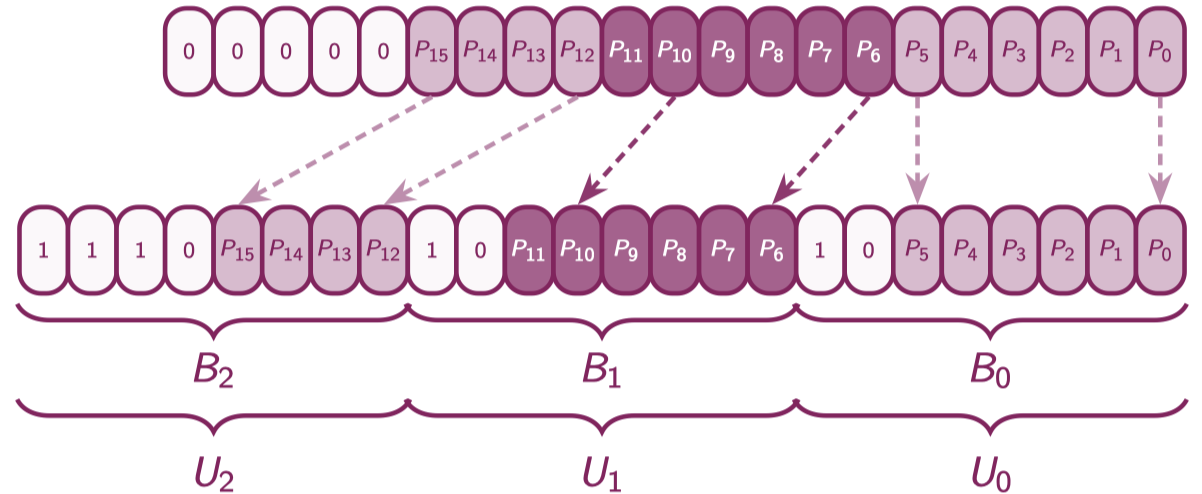
\includegraphics[scale=0.25]{UTF-8.png}
	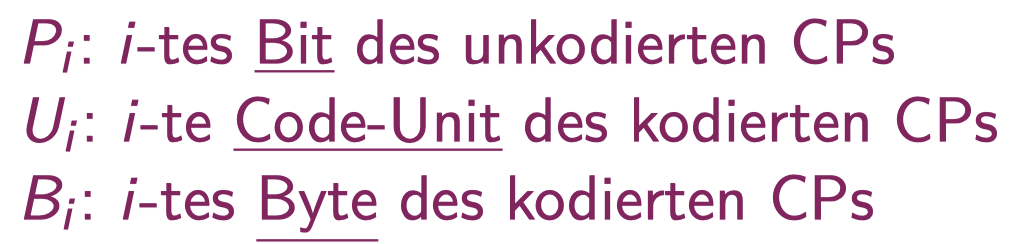
\includegraphics[scale=0.15]{UTF_Codierung_Begriffe.png}
	
	\textbf{UTF-16} CP in [0, FFFF] ohne [D800, DFFF] Ein \textbf{Surrogate Pair} besteht aus zwei Code Points, die ein einzelnes Zeichen repräsentieren. Der erste Code Point befindet sich im Bereich von D800 bis DBFF, während der zweite Code Point im Bereich von DC00 bis DFFF liegt.
	
	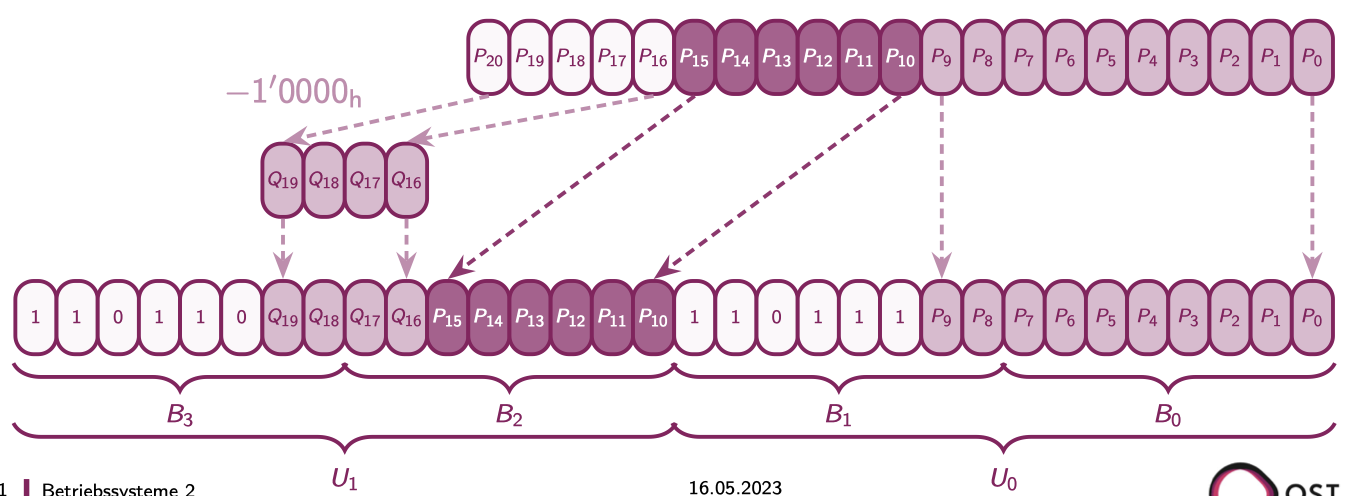
\includegraphics[scale=0.225]{UTF-16.png}%TODO noch anschauen

	\textbf{ext2} Begriffe: \underline{Partition} (Teil des Datenträgers, wird selbst wie Datenträter behandelt) \underline{Volume} (Ein Datenträger/Partition davon) \underline{Sektor} (Kleinste mögliche Untereinheit eines Volumes bis 4KB, Enthält Header, Daten und Error-Correction-Codes) \underline{Format} (Layout der logischen Struktur des Datenträgers)\\
	
	In einem \textbf{Block} sind mehrere Sektoren (1,2 oder 4KB). Volume ist in Blöcke aufgeteilt. Speicher wird nur in Form von Blöcken alloziert. Ein Block enthält nur Daten einer einzigen Datei.
	\begin{itemize} [noitemsep, topsep=0pt, leftmargin=*]
		\item \textbf{Logische} Blocknummer: Blocknummer vom Anfang der Datei aus gesehen, wenn Datei eine ununterbrochene Abfolge von Blöcken wäre
		\item \textbf{Physische} Blocknummer: Tatsächliche Blocknummer auf dem Volume
	\end{itemize}
	\vspace{5pt}
	Ein \textbf{Inode} ist die Bschreibung einer Datei, enthält alle Metadaten und hat Fixe Grösse je Volume: Zweierpotenz, mind. 128 Byte, max. 1 Block
	
	\vspace{5pt}
	\rule{\linewidth}{0.4pt}
	\textbf{[ext4]}\\
	
	\vspace{5pt}
	\rule{\linewidth}{0.4pt}
	\textbf{[X-Window-System]}\\
\end{multicols*}
\end{document}
